\documentclass[12pt]{article}
\usepackage{amsmath}
\usepackage{amssymb} % Required for \langle and \rangle
\usepackage{amsmath} % Required for \mid and other math symbols
\usepackage{listings}
\usepackage{color}
\usepackage{tikz} % Required for drawing diagrams like parse trees
\usetikzlibrary{trees,automata,positioning}
\usepackage{listing}
\usepackage{geometry}
\usepackage{float} % Required for the [H] float option
\usepackage{graphicx} % Required for including images
\geometry{margin=1in}
\usepackage{caption}
\usepackage[colorlinks=true, linkcolor=black, urlcolor=blue, citecolor=blue]{hyperref}
\usepackage{fancyhdr}
\usepackage{color}
\usepackage{xcolor} % Needed for custom colors
\definecolor{purple}{rgb}{0.5,0.0,0.5} % Define purple manually
\definecolor{codegray}{rgb}{0.5,0.5,0.5}
\definecolor{backcolour}{rgb}{0.95,0.95,0.92}


\pagestyle{fancy}
\fancyhead[L]{ Assignment -3 } 
\fancyhead[R]{ Gandholi Sarat - 23008 }
\title{\textbf{PMAT 402 - Systems Programming \\ Assignment -3 }}
\author{\textbf{Gandholi Sarat - 23008}}
\author{Gandholi Sarat - 23008}
\date{\today}

\definecolor{codegray}{rgb}{0.5,0.5,0.5}
\definecolor{backcolour}{rgb}{0.95,0.95,0.92}
\lstdefinestyle{mystyle}{
    backgroundcolor=\color{backcolour},   
    commentstyle=\color{codegray},
    keywordstyle=\color{blue},
    numberstyle=\tiny\color{codegray},
    stringstyle=\color{purple},
    basicstyle=\ttfamily\footnotesize,
    breakatwhitespace=false,         
    breaklines=true,                 
    captionpos=b,                    
    keepspaces=true,                 
    numbers=left,                    
    numbersep=5pt,                  
    showspaces=false,                
    showstringspaces=false,
    showtabs=false,                  
    tabsize=2
}
\lstset{style=mystyle}

\begin{document}

\renewcommand{\thesection}{Q\arabic{section}}


\maketitle
\tableofcontents
\newpage


% Question 1
\section{Write a sequence of instructions for SIC/XE to set ALPHA equal to 4*BETA - 9. Use immediate addressing for constants.}

To compute:

\[
\texttt{ALPHA = 4 * BETA - 9}
\]

in SIC/XE, we follow these steps:

\begin{enumerate}
    \item Load the value stored at \texttt{BETA}.
    \item Multiply it by 4 using immediate addressing.
    \item Subtract 9 using immediate addressing.
    \item Store the result in \texttt{ALPHA}.
\end{enumerate}

\textbf{Instruction Sequence:}

\begin{lstlisting}[language={[x86masm]Assembler}]
        LDA     BETA       ; Load value of BETA into accumulator A
        MUL     #4         ; Multiply A by 4 (immediate)
        SUB     #9         ; Subtract 9 from A (immediate)
        STA     ALPHA      ; Store result into ALPHA
\end{lstlisting}

\textbf{Data Declarations:}

\begin{lstlisting}[language={[x86masm]Assembler}]
ALPHA   RESW    1          ; Reserve 1 word for ALPHA
BETA    WORD    5          ; Example value: BETA = 5
\end{lstlisting}

\textbf{Explanation:}

\begin{itemize}
    \item \texttt{LDA BETA} loads the content of memory location \texttt{BETA} into register A.
    \item \texttt{MUL \#4} multiplies A by 4 using immediate addressing.
    \item \texttt{SUB \#9} subtracts the constant 9.
    \item \texttt{STA ALPHA} stores the final result into \texttt{ALPHA}.
\end{itemize}

This sequence assumes the program is running in SIC/XE mode with support for immediate addressing and that appropriate directives (such as \texttt{START}, \texttt{END}) and base register setup are present elsewhere in the program if needed.



\newpage
% Question 2
\section{Write SIC instruction to swap the values ALPHA and BETA.}

To swap the values of two memory locations \texttt{ALPHA} and \texttt{BETA} in SIC (Standard Instruction Computer), we need a temporary location to hold one of the values during the swap.

\textbf{Instruction Sequence:}

\begin{lstlisting}[language={[x86masm]Assembler}]
        LDA     ALPHA       ; Load value of ALPHA into A
        STA     TEMP        ; Store it in TEMP

        LDA     BETA        ; Load value of BETA into A
        STA     ALPHA       ; Store it into ALPHA

        LDA     TEMP        ; Load original ALPHA from TEMP
        STA     BETA        ; Store it into BETA
\end{lstlisting}

\textbf{Data Declarations:}

\begin{lstlisting}[language={[x86masm]Assembler}]
ALPHA   WORD    10          ; Example value
BETA    WORD    20          ; Example value
TEMP    RESW    1           ; Temporary word for swapping
\end{lstlisting}

\textbf{Explanation:}
\begin{itemize}
    \item Load \texttt{ALPHA} into register A and store it in \texttt{TEMP}.
    \item Load \texttt{BETA} and store it into \texttt{ALPHA}.
    \item Load the original value of \texttt{ALPHA} from \texttt{TEMP} and store it into \texttt{BETA}.
\end{itemize}

This correctly swaps the values in memory locations \texttt{ALPHA} and \texttt{BETA} using a simple temporary variable and only the accumulator (A), which is typical in SIC programming.


% Add the output table here (as created earlier with \begin{tabularx}...)
\newpage
% Question 3
 \section{Draw parse trees according to the grammar for the following $\langle \exp \rangle$:}

\textbf{Expression:} \texttt{ALPHA - BETA * GAMMA}

\bigskip

\textbf{Grammar Rules:}

\begin{itemize}
    \item $\langle \text{exp} \rangle \rightarrow \langle \text{exp} \rangle\ -\ \langle \text{term} \rangle\ |\ \langle \text{term} \rangle$
    \item $\langle \text{term} \rangle \rightarrow \langle \text{term} \rangle\ *\ \langle \text{factor} \rangle\ |\ \langle \text{factor} \rangle$
    \item $\langle \text{factor} \rangle \rightarrow \texttt{id} \ |\ \texttt{int} \ |\ (\langle \text{exp} \rangle)$
\end{itemize}


\bigskip

\textbf{Parse Tree:}

\begin{center}
    \begin{tikzpicture}[level distance=1.5cm,
      every node/.style={draw, rectangle, align=center},
      level 1/.style={sibling distance=6cm},
      level 2/.style={sibling distance=4cm},
      level 3/.style={sibling distance=2.5cm}
    ]
    
    \node {$\langle \text{exp} \rangle$}
        child {node {$\langle \text{exp} \rangle$}
            child {node {$\langle \text{term} \rangle$}
                child {node {$\langle \text{factor} \rangle$}
                    child {node {ALPHA}}
                }
            }
        }
        child {node {-}}
        child {node {$\langle \text{term} \rangle$}
            child {node {$\langle \text{term} \rangle$}
                child {node {$\langle \text{factor} \rangle$}
                    child {node {BETA}}
                }
            }
            child {node {*} }
            child {node {$\langle \text{factor} \rangle$}
                child {node {GAMMA}}
            }
        };
    \end{tikzpicture}
\end{center}

\textbf{Explanation:} According to the grammar and operator precedence, multiplication is performed before subtraction. Hence, the expression is grouped as:

\[
\texttt{ALPHA - (BETA * GAMMA)}
\]

The parse tree reflects this structure by breaking down the expression first by `-` at the top level and then by `*` within the right subtree.


% Optionally: insert TikZ trees here, or draw manually and include as an image
\newpage
% Question 4
\section{Draw FSM to recognize a token type named \texttt{Real constant}.}

A real constant may contain digits and must either include a decimal point or a scale factor (or both). The scale factor consists of the letter \texttt{E} followed by a positive or negative integer. There must be at least one digit before the decimal point (if any).

\begin{center}
    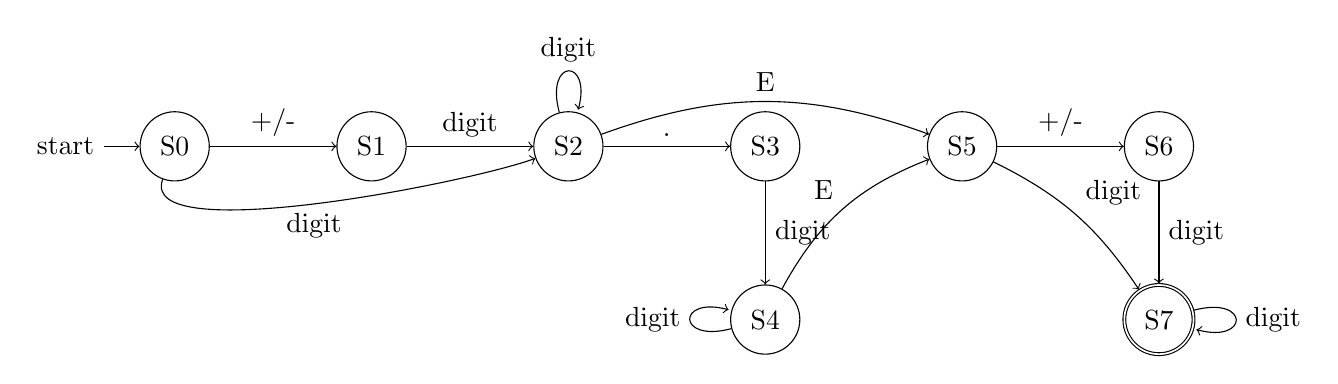
\begin{tikzpicture}[->, node distance=2.2cm and 2.5cm, on grid, auto]
    
      % States
      \node[state, initial] (Sstart) {S0};
      \node[state] (S0) [right=of Sstart] {S1};
      \node[state] (S1) [right=of S0] {S2};
      \node[state] (S2) [right=of S1] {S3};
      \node[state] (S3) [below=of S2] {S4};
      \node[state] (S4) [right=of S2] {S5};
      \node[state] (S5) [right=of S4] {S6};
      \node[state, accepting] (S6) [below=of S5] {S7};
    
      % Transitions
      \path
        (Sstart) edge node {+/-} (S0)
        (Sstart) edge[out=250, in=200, looseness=.5] node[below] {digit} (S1)
    
        (S0) edge node {digit} (S1)
    
        (S1) edge [loop above] node {digit} (S1)
        (S1) edge node {.} (S2)
        (S1) edge[bend left=20] node {E} (S4)
    
        (S2) edge node {digit} (S3)
        (S3) edge [loop left] node {digit} (S3)
        (S3) edge[bend left=20] node {E} (S4)
    
        (S4) edge node {+/-} (S5)
        (S4) edge[bend left=15] node {digit} (S6)
    
        (S5) edge node {digit} (S6)
        (S6) edge [loop right] node {digit} (S6);
    
    \end{tikzpicture}
    \end{center}
    


% Optionally: draw FSM using TikZ or include scanned FSM image
\newpage
% Question 5
\section{What are the different classes of interrupts and their corresponding types in SIC/XE architecture? Explain with code examples.}

The SIC/XE architecture supports different classes of interrupts that are triggered by software or hardware events. Each class is designed for specific types of operations such as system calls, error handling, timing, or I/O operations.

\begin{center}
    \begin{tabular}{|c|l|}
    \hline
    \textbf{Class} & \textbf{Interrupt Type} \\
    \hline
    I   & Supervisor Call (SVC) \\
    II  & Program Interrupt \\
    III & Timer Interrupt \\
    IV  & I/O Interrupt \\
    \hline
    \end{tabular}
    \end{center}
    
    \vspace{0.2cm}
    
    \subsection*{Class I: Supervisor Call (SVC)}
    
    Class I interrupts are generated by executing the \texttt{SVC} instruction. These are software interrupts used to request privileged operations or services from the operating system, such as file I/O, memory management, or printing data.
    
    \textbf{Use Case:} When a program requires access to protected resources or services, it uses an \texttt{SVC} call. The OS provides the appropriate handler for each service ID.
    
    \textbf{Example: Request to print a character}
    
    \begin{lstlisting}[language={[x86masm]Assembler}]
    LDA     CHAR        ; Load character to be printed
    SVC     1           ; Request OS to print character
    ...
    CHAR    BYTE    C'A'
    \end{lstlisting}
    
    \textit{Explanation:} The \texttt{SVC 1} call causes a trap to the operating system, transferring control to the interrupt handler associated with service 1. The OS then accesses the character in register A and sends it to the output device.
    
    \vspace{0.2cm}
    
    \subsection*{Class II: Program Interrupt}
    
    Class II interrupts occur due to illegal or exceptional operations during program execution, such as division by zero, invalid instructions, or memory access violations. These interrupts are used to detect and handle errors.
    
    \textbf{Use Case:} Error detection and graceful failure handling during abnormal program behavior.
    
    \textbf{Example: Divide by zero error (simulated)}
    
    \begin{lstlisting}[language={[x86masm]Assembler}]
    LDA     NUM1        ; Load numerator
    DIV     NUM0        ; Attempt division by zero
    STA     RESULT
    ...
    NUM1    WORD    10
    NUM0    WORD    0    ; Division by zero causes Class II interrupt
    \end{lstlisting}
    
    \textit{Explanation:} The division operation checks if the divisor is zero. If true, a program interrupt is generated, which halts execution and passes control to an error handler routine to prevent a crash or undefined behavior.
    
    \vspace{0.2cm}
    
    \subsection*{Class III: Timer Interrupt}
    
    Class III interrupts are generated by a hardware timer, commonly used to implement multitasking, preemptive scheduling, or system resource monitoring. The timer interrupt helps enforce time-sharing between processes.
    
    \textbf{Use Case:} Allow the OS to regain control after a time quantum expires, facilitating CPU scheduling.
    
    \textbf{Example: Simulated scheduling interrupt after time slice}
    
    \begin{lstlisting}[language={[x86masm]Assembler}]
    START   LDA     #0
    LOOP    ADD     #1
            COMP    #1000
            JLT     LOOP     ; Loop until 1000 iterations
            ...              ; Timer overflows => Class III interrupt
    \end{lstlisting}
    
    \textit{Explanation:} Although not explicitly triggered in code, a hardware timer running in the background can interrupt the loop when the allocated time expires. The OS then uses this interrupt to perform scheduling or context switching.
    
    \vspace{0.2cm}
    
    \subsection*{Class IV: I/O Interrupt}
    
    Class IV interrupts occur when an I/O operation completes or when a device requires CPU attention. These interrupts allow asynchronous communication between the processor and peripheral devices.
    
    \textbf{Use Case:} Efficient I/O handling without polling; devices signal when ready, freeing CPU cycles.
    
    \textbf{Example: Read data from device}
    
    \begin{lstlisting}[language={[x86masm]Assembler}]
    TD      DEVICE      ; Test device
    JEQ     WAIT        ; If device not ready, wait
    RD      DEVICE      ; Read from device
    STCH    BUFFER      ; Store character in buffer
    ...
    DEVICE  BYTE    X'F1'
    BUFFER  RESB    1
    \end{lstlisting}
    
    \textit{Explanation:} The device signals readiness using the \texttt{TD} instruction. Once ready, the \texttt{RD} instruction reads data, and an I/O interrupt is generated upon completion. The OS then transfers control to an I/O handler that processes the incoming data and resumes normal execution.
\end{document}
